I fliken \verb+Lägg till/Uppdatera recept+ finner du all funktionalitet som har att göra med att lägga till och uppdatera recept. För att lägga till ett recept från en extern källa så som en bok följer man följande steg i godtycklig ordning, förutom det allra sista steget som måste ske sist. 

\begin{figure}[H]
        \centering 
        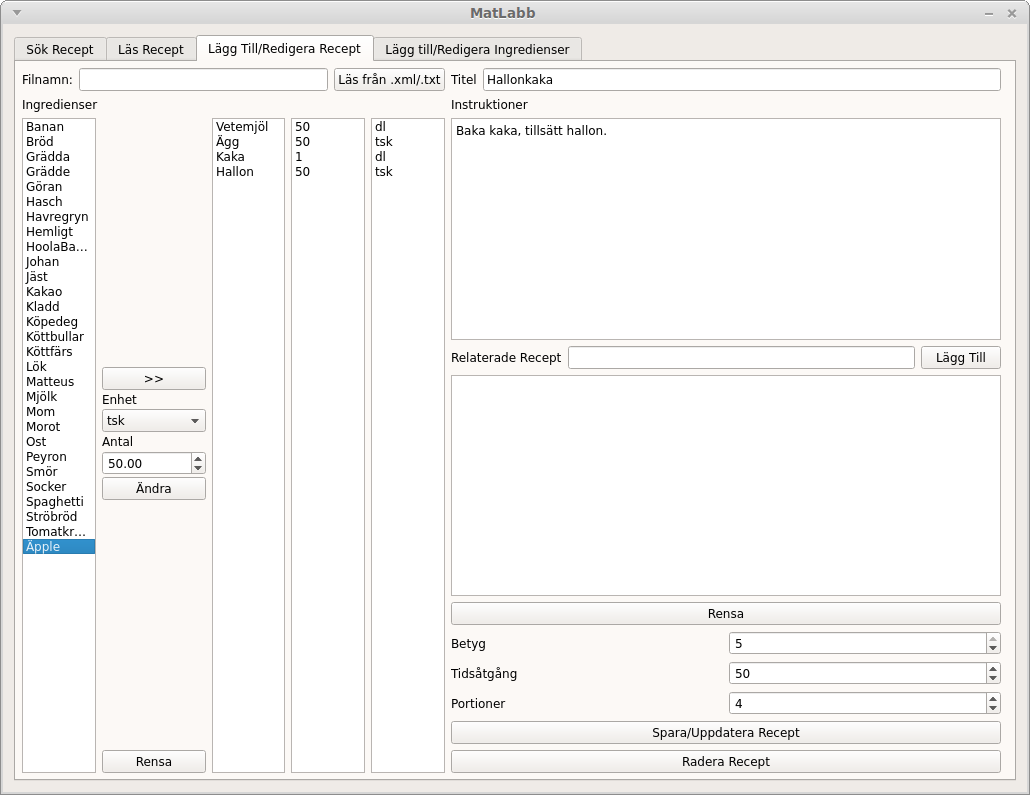
\includegraphics[scale=0.44]{lagg_till_recept.png} 
        \caption{Lägg till/Redigera Recept} 
        \label{fig:laggtillreceptvyn}
\end{figure}

\begin{itemize}
\item Steg 1: Fyll i en titel som är unik för ditt recept. Fyller du i en titel på ett recept som redan finns sparat så kommer detta recept sparas över med ny information.
\item Steg 2: Markera en ingrediens i kollumen till vänster. Ange information om vilken mängd och måttenhet som ingrediensen skall användas i. Klicka sedan på knappen \verb+>>+ för att lägga till ingrediensen i receptet. Upprepa detta tills alla ingredienser som krävs för receptet är angivna .
\em Om misstag sker vid inmatning, exempelvis om man råkar ange fel måttenhet eller mängd kan detta enkelt fixas. Markera ingrediensen i kollumnen med ingredienser, fyll i rätt måttenhet och mängd i fälten mellan kollumnerna, och klicka på knappen \verb+Ändra+. 
Om väldigt många misstag sker vid inmatning, så kan knappen "Rensa" användas för att ta bort alla ingredienser från receptet, då finns möjlighet att börja om från början och försöka göra inmatningen igen. \em
\item Steg 3: Finns det relaterade recept till ditt recept? Fyll då i titlarna i fältet "Relaterade Recept", en efter en, och klicka på knappen \verb+Lägg Till+ emellan. Dessa titlar kommer nu visas i en lista alldeles under fältet. Dessa recept kommer man enkelt att hitta när man sedan öppnar det här receptet. Knappen \verb+Rensa+ tömmer den här listan. 
\item Steg 4: Fyll i ett betyg. Detta kan göras senare då man lagat receptet och vet hur man skulle betygsätta det. 
\item Steg 5: Fyll i uppskattad tidsåtgång.
\item Steg 6: Fyll i hur många portioner som receptet är skrivet till. 
\item Steg 7: Klicka på \verb+Spara/Uppdatera Recept+ receptet finns nu sparat, det går att söka på och öppna. 
\end{itemize}

\subsection{Import av recept från fil}
För att mata in ett recept via .txt eller .xml-fil, så placeras filen i samma map som MatLabb ligger i. Skriv sedan filnamnet i fältet \verb+Filnamn+, och klicka på knappen \verb+Läs från .txt/.xml+. Matlabb kommer då att fylla i alla fält för att lägga till recept baserat på vad som finns i filen. Det återstår då för dig att kontrollera att inläsningen skett korrekt, gör eventuella korrigeringar, och klicka sedan på \verb+Spara/Uppdatera Recept+.


